\documentclass[11pt]{article}

\usepackage{float}
\usepackage{hyperref}
\usepackage{fullpage}
\usepackage{verbatim}
\usepackage{moreverb}
\usepackage{graphicx}
\usepackage{parskip}
\usepackage{amsmath}
\usepackage[toc,page]{appendix}
\graphicspath{{images/}}
\usepackage{gensymb}

\usepackage{minted}
\let\verbatiminput=\verbatimtabinput
\def\verbatimtabsize{4\relax}

\begin{document}
\title{EE 241B HW3 Writeup}

\author{Vighnesh Iyer}
\date{}
\maketitle

\tableofcontents

\section{Building and Characterizing a Standard Cell}

\subsection{Flow and Decoder Delay Using Custom Cell}
We go through the tutorial to design a custom NAND2 standard cell. We first record the critical path of the 3-8 decoder used in the previous lab with the NAND2 cell supplied with the design kit. The critical path goes from \verb|A[3]| to \verb|Z[5]| and it has a delay of 0.1376 ns.

We then tell DC and ICC to use our custom standard cell and we measure the critical path again. The critical path now goes from \verb|A[0]| to \verb|Z[14]| and has a delay of 0.1019 ns, which is an improvement over the previous ICC run. However, looking at the final Verilog netlist from ICC only 2 instances of our \verb|NAND2X1B_RVT| cell exist. However, after running only DC, there were many instances of our custom cell. It seems that ICC did some optimization and swapped out most of those custom cells for standard cells from the design kit.

\begin{figure}[H]
	\centerline{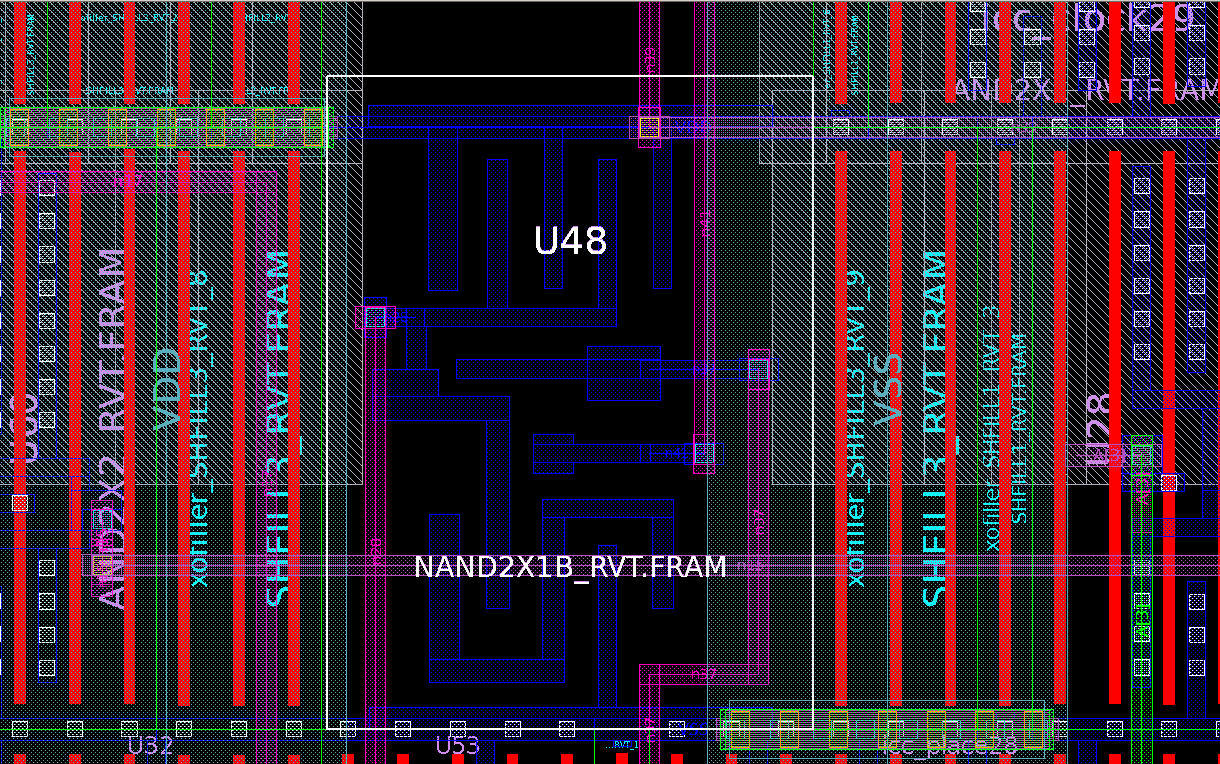
\includegraphics[height=7cm]{icc_custom_cell.png}}
	\caption{An instance of the NAND2X1B\_RVT cell in ICC with visible M1 polygons.}
\end{figure}

\subsection{Standard Cell Inverter Variation Impact vs $V_{DD}$}
We run a 300 point Monte Carlo simulation and plot the mean and sigma for the input-rising/output-falling delay of the \verb|INVX0_RVT| standard cell for $V_{DD}$ between 0.2 and 1.05. We fix an input slope of 10ps and a 1fF load. This part was done by exporting a netlist from Virtuoso and using commandline HSPICE for the simulation.

\begin{figure}[H]
	\centerline{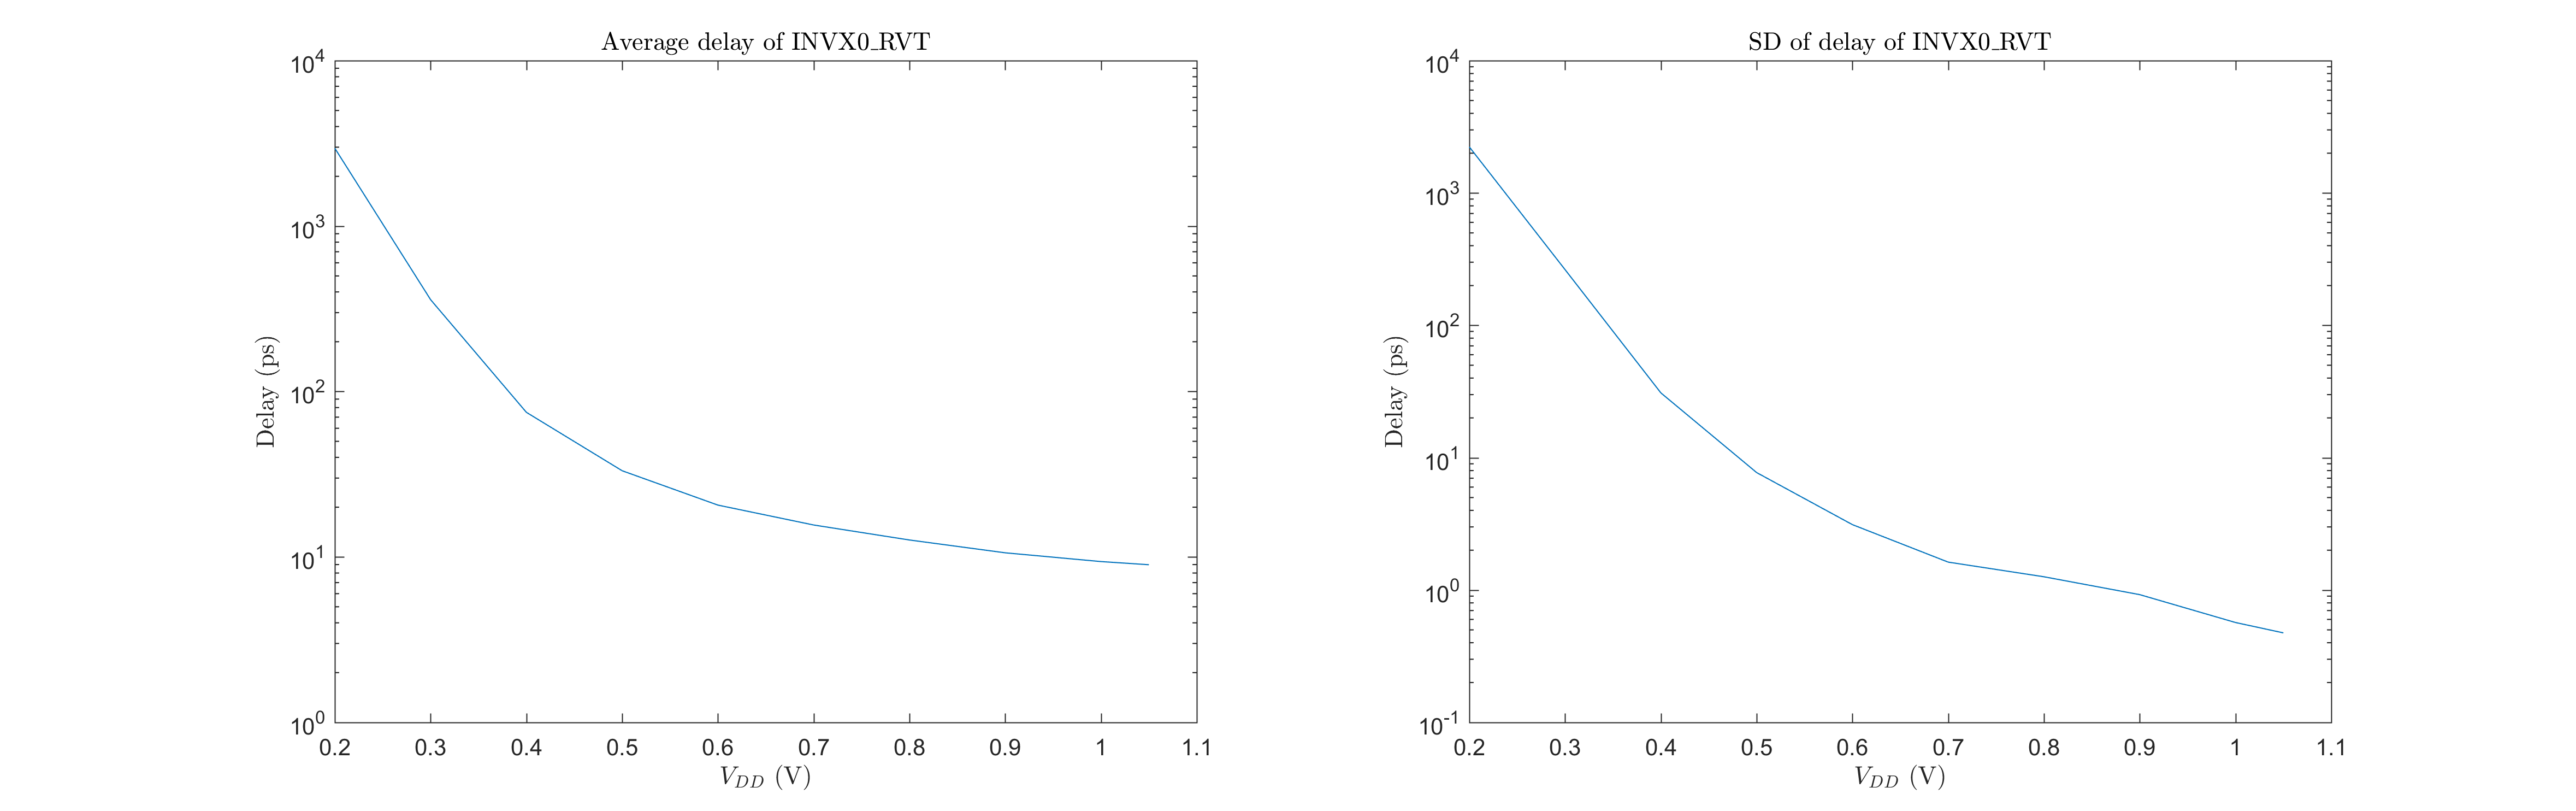
\includegraphics[width=\textwidth+4cm]{delay_vs_vdd.png}}
	\caption{Plot is log-scale in y-axis.}
\end{figure}

We then plot $\sigma / \mu$ vs. $V_{DD}$.

\begin{figure}[H]
	\centerline{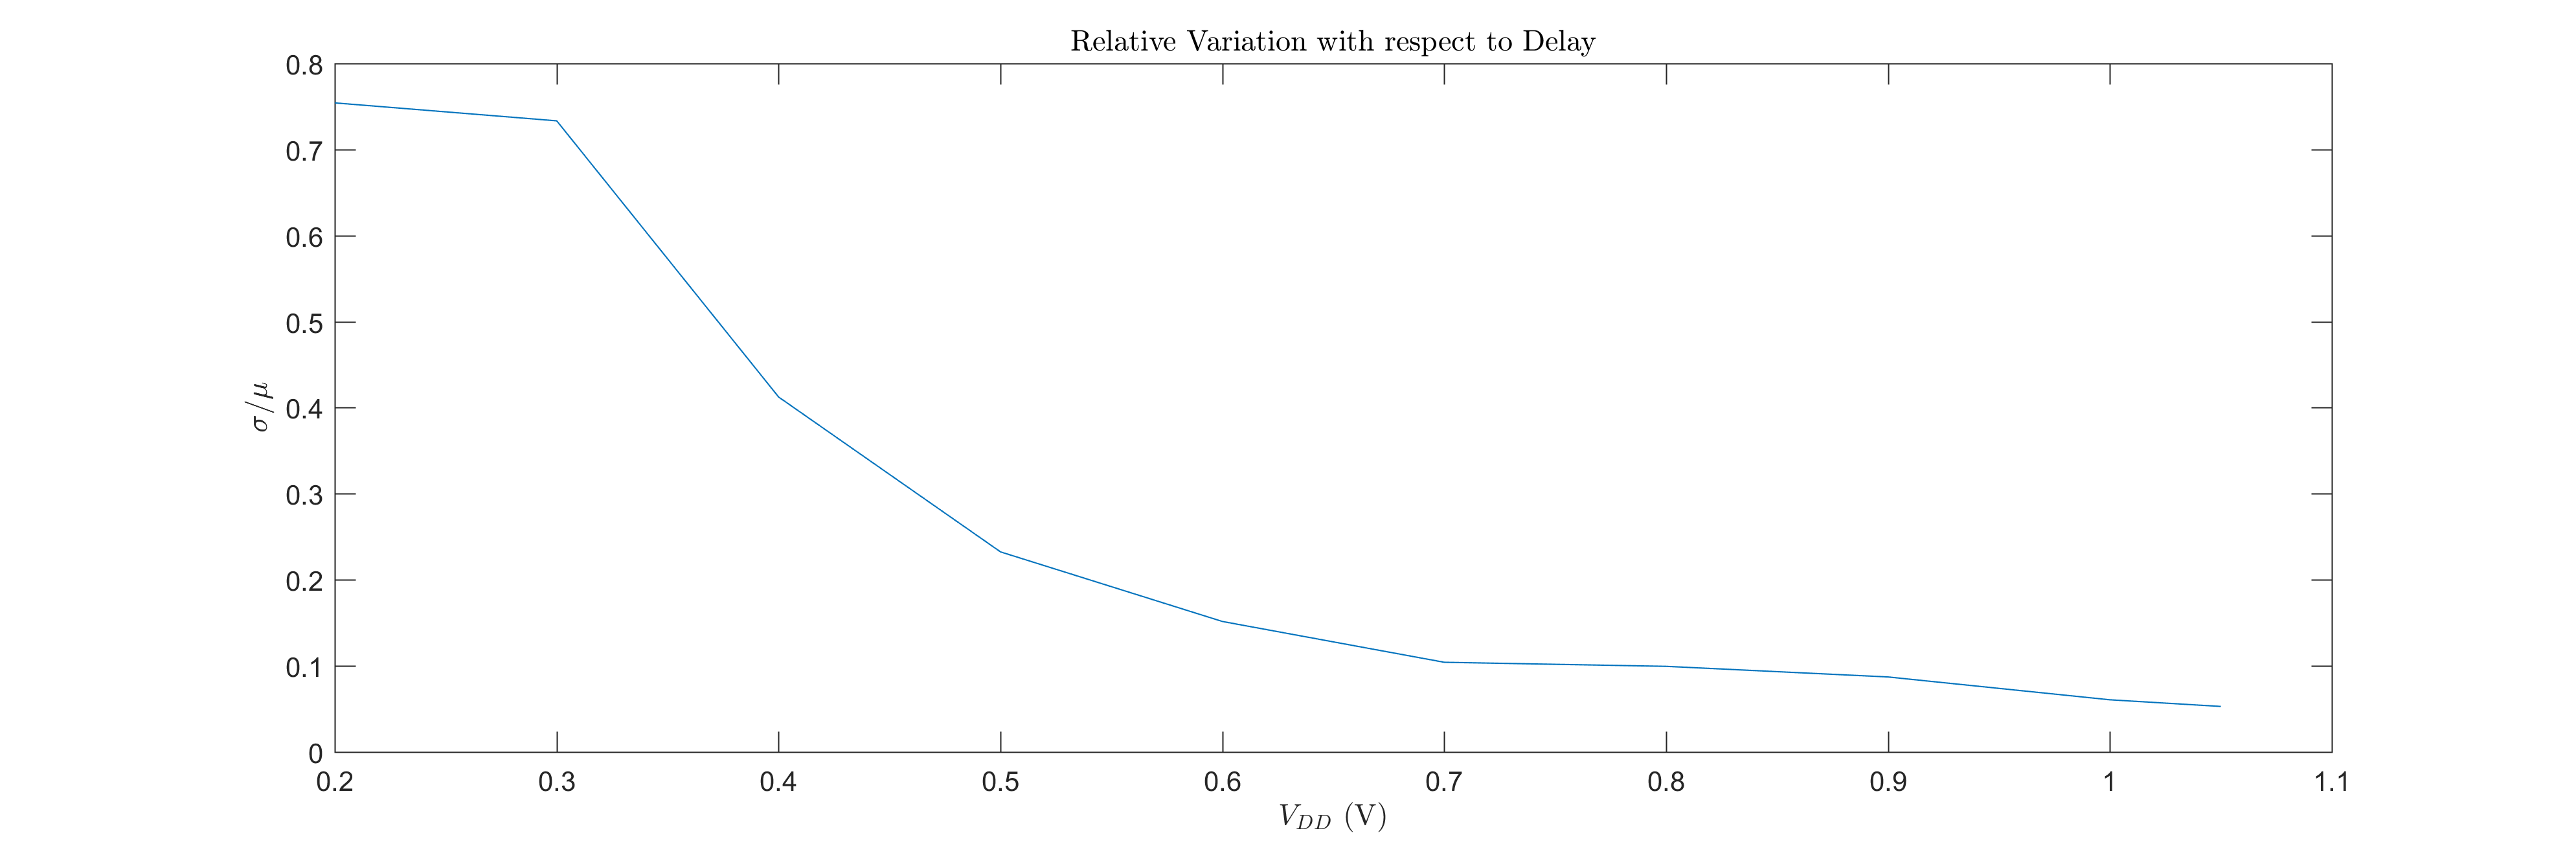
\includegraphics[width=\textwidth+4cm]{relative_delay_variation_vs_vdd.png}}
\end{figure}

Finally we plot the delay of a $6 \sigma$ cell relative to the mean vs. $V_{DD}$.

\begin{figure}[H]
	\centerline{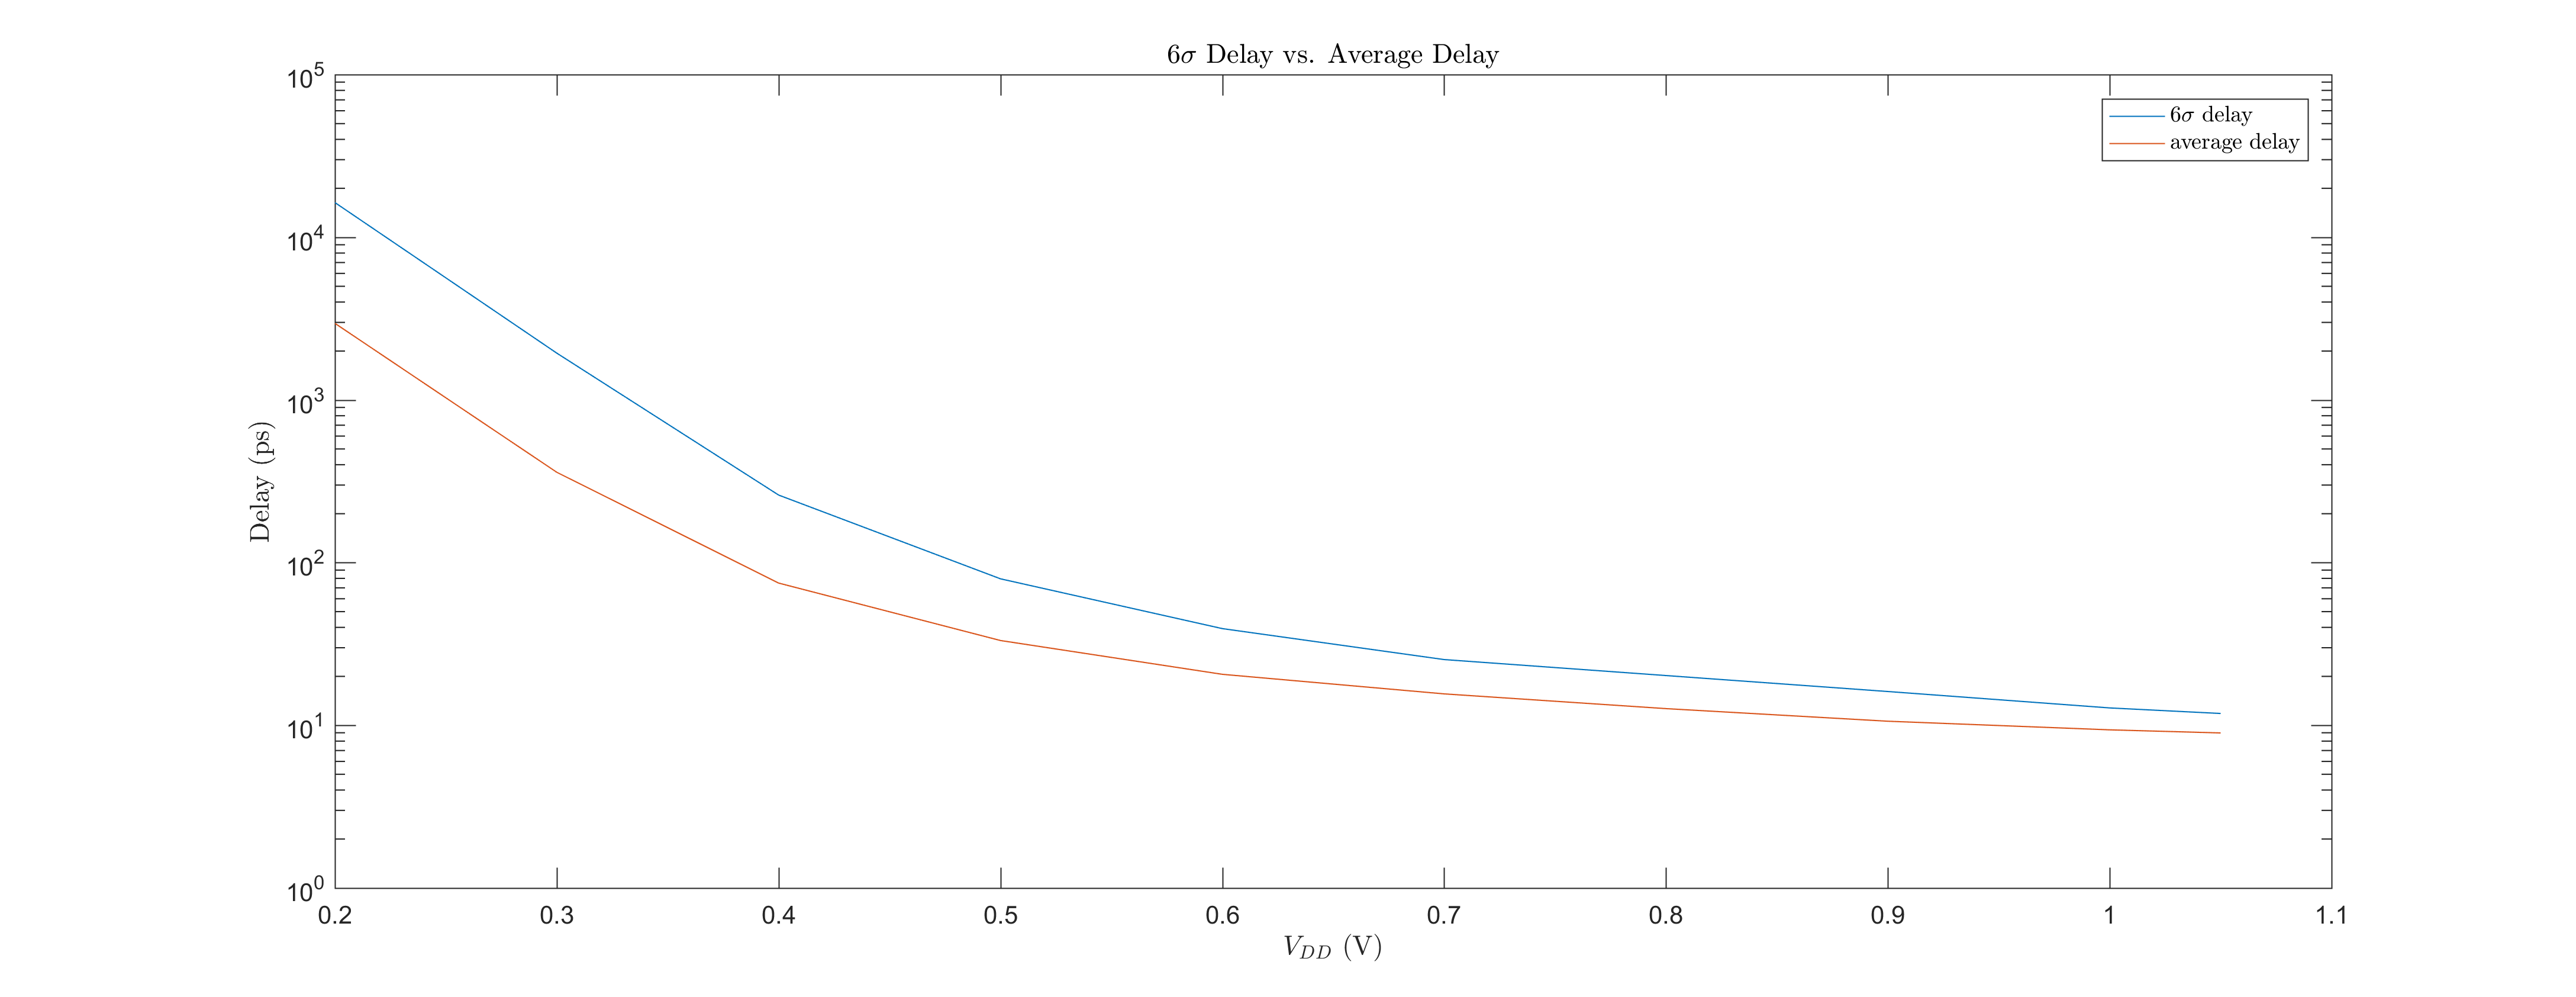
\includegraphics[width=\textwidth+4cm]{six_sigma_delay_vs_vdd.png}}
\end{figure}

Variation has a larger effect at low voltages since our mismatch model works by setting $V_{th}$ of each transistor using a probability distribution with a $\sigma_{V_{th}}$. At lower voltages, the transistor has an operating voltage around its threshold voltage and thus makes the variation more pronounced.

\subsection{Delay Distributions for Different $V_{DD}$}
We create histograms and fit a normal curve for the delay at 0.6V and 1.05V. 

\begin{figure}[H]
	\centerline{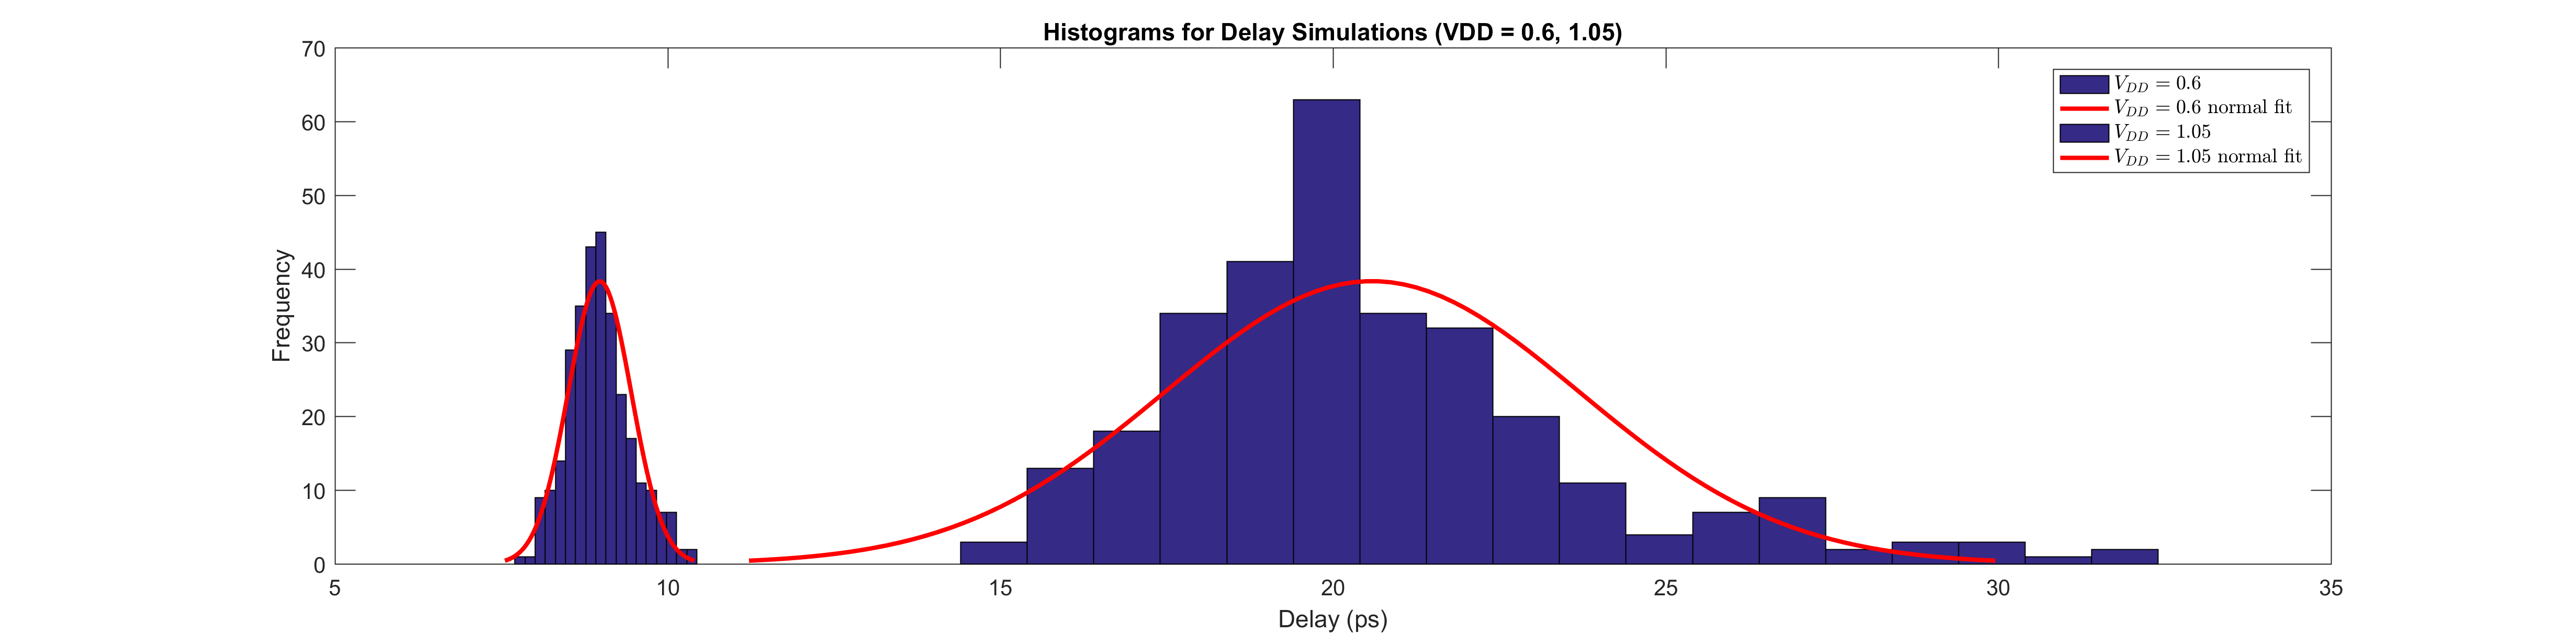
\includegraphics[width=\textwidth+4cm]{delay_histograms.png}}
	\caption{Two histograms that contain delays from the 300 point monte carlo sim. Left histogram is at $V_{DD} = 1.05V$ and right histogram is at $V_{DD} = 0.6V$.}
\end{figure}

The histogram for $V_{DD} = 1.05V$ is roughly Gaussian and can be closely approximated with a normal distribution. However the histogram for $V_{DD} = 0.6V$ is asymmetric and a Gaussian is a poor fit for it. There is a long right tail, and it comes about due to a certain transistor having a much higher $V_{th}$ which increases its delay a lot more at a lower $V_{DD}$.

\subsection{$\sigma_{V_{th}}$ and Monte Carlo in MATLAB}
We compute $\sigma_{V_{th}}$ for the NMOS in \verb|INVX0_RVT|. As per the Pelgrom mismatch model:

\begin{equation}
	\sigma_{V_{th}} = \frac{A_{V_t}}{\sqrt{W \cdot L}} = \frac{2}{\sqrt{W \cdot L \cdot 1e6 \cdot 1e6}} \text{ mV}
\end{equation}

In this design kit, $A_{V_t}$ is set to 2 $mV \cdot \mu m$. The minimally sized inverter contains an NMOS with a width of 520nm and length of 30nm. Thus, we get $\sigma_{V_{th}} = 16.01$ mV for the NMOS.

Now we use the alpha-power law's equation for $I_{on}$ and parameter values $K = 1.7\text{e-4}, V_{th} = 0.336, \alpha = 1.36$. We find the equation for the delay of an inverter assuming maximum current for a transition from $V_{DD}$ to $V_{DD}/2$. We also estimate $\Delta T = C \Delta V / I$ where $\Delta V = V_{DD} / 2$ and $C \approx 1.5$ fF.

\begin{eqnarray}
	I_{on} = K (V_{gs} - V_{th}) ^ \alpha \nonumber \\
	\Delta T = \frac{C \cdot 0.5 V_{DD}}{K (V_{DD} - V_{th} + \Delta V_{th}) ^ \alpha} \nonumber
\end{eqnarray}

We use MATLAB to run a Monte Carlo simulation on this delay model for $V_{DD} = 0.5, 1.05$ V and compare it with the HSPICE results in the previous section. We get 600 samples from a (0, $\sigma_{V_{th}}$) normal distribution and plug those samples into the delay formula for different values of $V_{DD}$.

\begin{figure}[H]
	\centerline{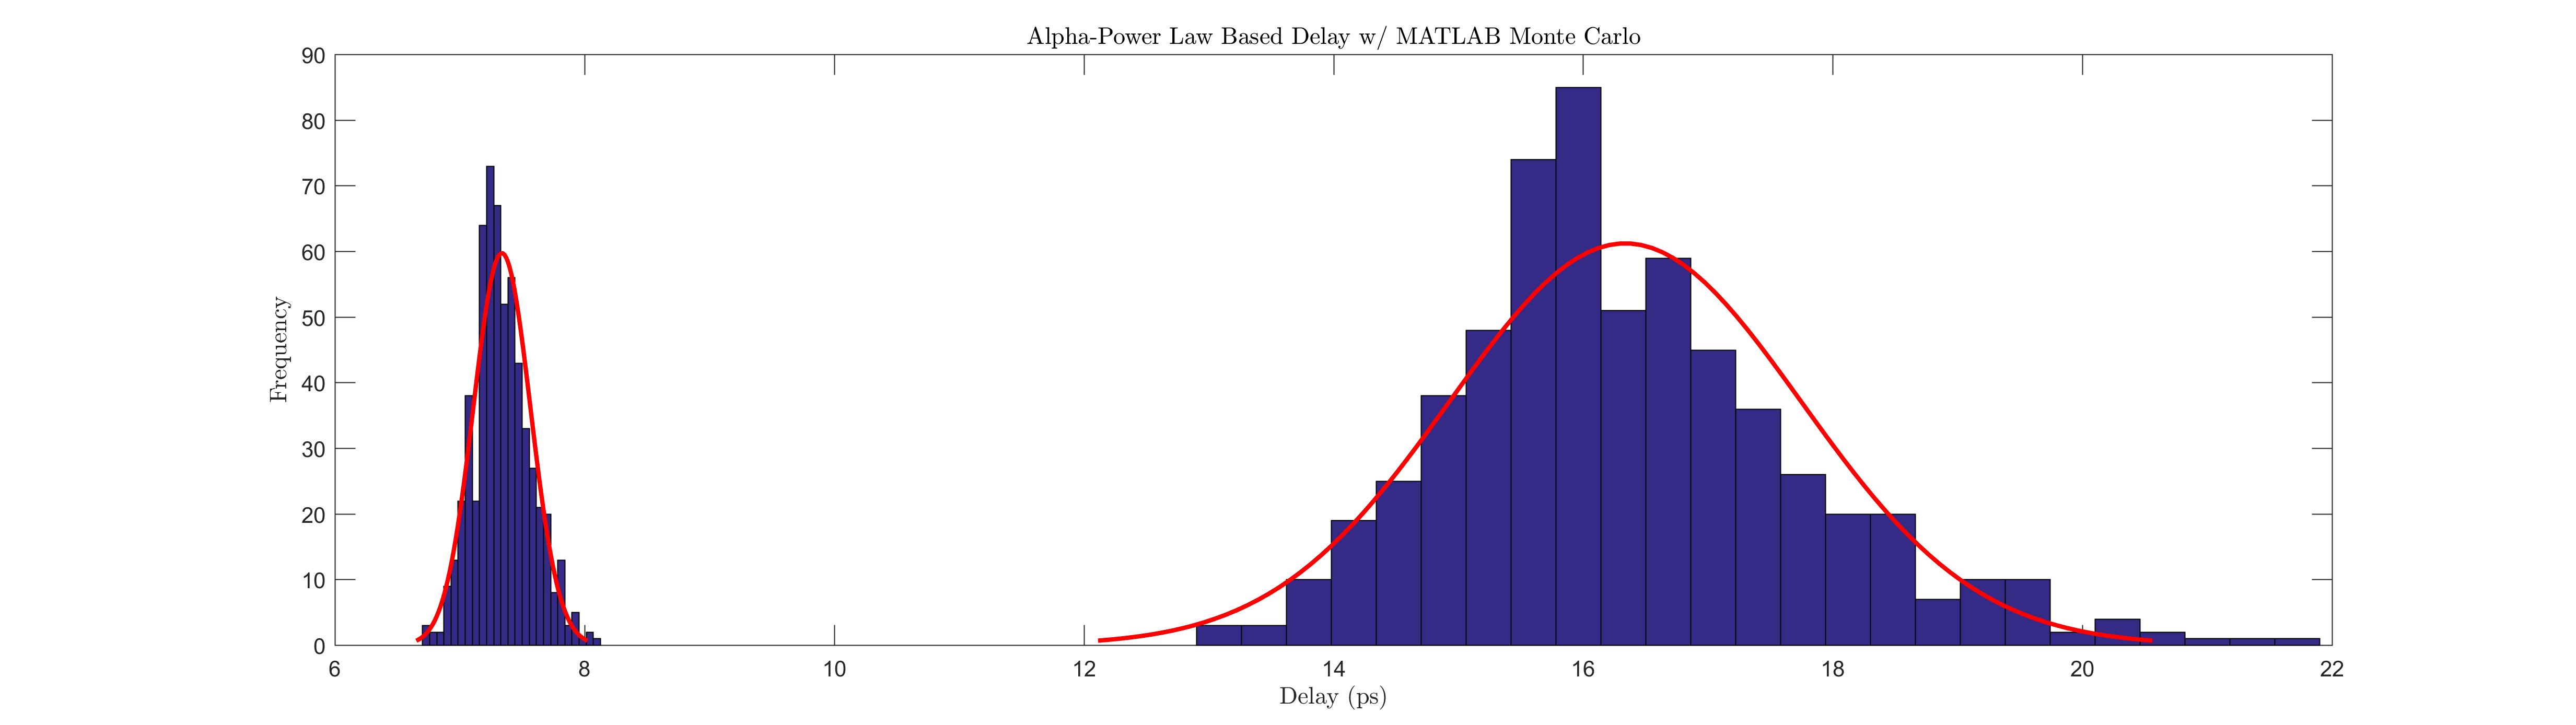
\includegraphics[width=\textwidth+4cm]{delay_histograms_matlab.png}}
	\caption{Two histograms that contain delays from the MATLAB monte carlo sim (600 points). Left histogram is at $V_{DD} = 1.05V$ and right histogram is at $V_{DD} = 0.6V$.}
\end{figure}

We see similar output from the MATLAB Monte Carlo and the HSPICE Monte Carlo. The delay distribution for $V_{DD} = 1.05$V is narrow and approximately normal, while the delay distribution for $V_{DD} = 0.6$V is much wider and has a long right tail. Based on the delay equation, the distribution should approach a Gaussian with increasing $V_{DD}$.

\section{Flip-Flops}
\begin{figure}[H]
	\centerline{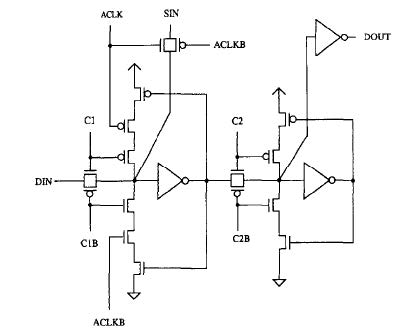
\includegraphics[height=5cm]{flip_flop_schematic.jpg}}
	\caption{A schematic of a sequential circuit.}
\end{figure}

\subsection{Identify Circuit}

Assuming that C1 and C2 are opposite phases of the same clock, the circuit above implements a \textbf{D-type flip-flop} using a master-slave latch topology.

When C1 is high, the first transmission gate is transparent and the data is allowed to settle at the input of the second transmission gate. At the moment that C2 goes high, C1 goes low to close off any further input changes, and the output reflects the 'last' value that passed through the first transmission gate while C1 was high.

The rest of the circuitry serves to make the flip-flop static by providing feedback into the storage nodes and there is an additional transmission gate that can be used by a scan chain.

\subsection{FF Timing Characteristics}
Assuming that the NMOS and PMOS devices have the same mobility and are all symmetrically sized, order the following timing parameters by magnitude: setup time, hold time, clock-output delay.

The setup time is approximately equal to the time it takes for an input signal at \verb|DIN| to race past the first transmission gate, after which the gate can become opaque. The hold time is close to 0 since after C2 goes high the first transmission gate becomes opaque and \verb|DIN| can't influence the flip-flop anyways. Also, the storage node doesn't need \verb|DIN| after the rising edge of C2. The clock to output delay is approximately equal to the delay through the second transmission gate and an inverter.

So in order of smallest to largest: \textbf{hold time, setup time, clock to output delay}.

\section{Timing}
\begin{figure}[H]
	\centerline{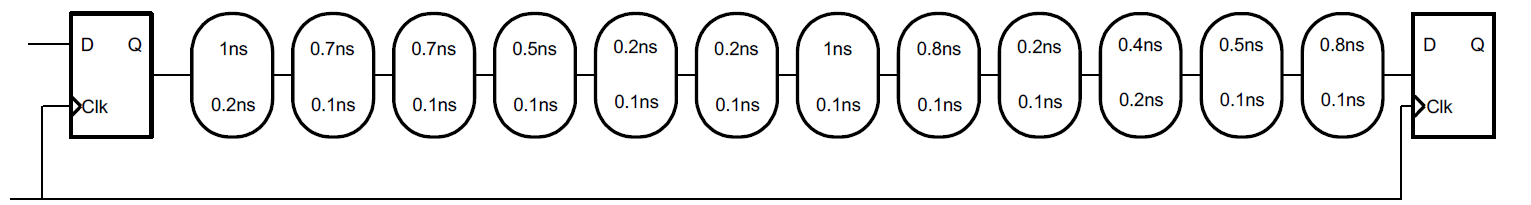
\includegraphics[width=\textwidth+4cm]{problem3_timing_path.png}}
\end{figure}

Given this pipeline stage and the annotated max and min propagation delays, we want to minimize the cycle time using deeper pipelining. An additional 2 cycles of latency can be added using either latches or FFs. Assume no clock skew. Clock duty cycle is fixed at 50\%.

\begin{itemize}
	\item FF: Clk-q = 200ps, Setup = 100ps, Hold = 0ps
	\item Latch: Clk-q, D-q = 150ps, Setup 100ps, Hold = 0ps
\end{itemize}

As the pipeline stage stands now, the minimum clock period is $T_{clk} = t_{clk-q} + t_{logic,max} + t_{setup} = 0.2 + 7.0 + 0.1 = 7.3$ns.

If we were to add 2 flip-flops, the goal is to divide the combinational delay equally between every flip-flop. This means a delay of $7.0/3 = 2.33$ns per stage. Failing to do that, the next best option would be placement of the flip-flops such that the maximum logic path between any 2 flip-flops is as short as possible. We can ignore hold time constraints since there is a positive $t_{clk-q}$ and zero hold time.

To iterate through the various placements of flip-flops, I wrote a script that's attached in the appendix. There are 3 flip-flop positions that obtain the minimal max delay among all 3 timing paths of 2.7 ns (leading to a minimum clock period of 3.0ns).

\begin{itemize}
	\item FF1 after 2 bubbles, FF2 after 7 bubbles, delays: (1.7, 2.6, 2.7)
	\item FF1 after 3 bubbles, FF2 after 7 bubbles, delays: (2.4, 1.9. 2.7)
	\item FF1 after 3 bubbles, FF2 after 8 bubbles, delays: (2.4, 2.7, 1.9)
\end{itemize}

We can likely improve on this clock period using latches to let the stage with longer delay borrow slack from the stage with shorter delay. For this to work optimally, the max difference between any two delays needs to be minimal. The 2nd or 3rd FF configuration is suitable for latch conversion. For latch timing analysis, we now need to look at hold time constraints as well.



\newpage
\appendix

\section{Inverter Delay vs. VDD SPICE File}
\begin{minted}[breaklines,tabsize=2]{text}
Running Monte-Carlo simulation while sweeping VDD

.lib '/home/ff/ee241/synopsys-32nm/hspice/saed32nm.lib' TT
*  Library name: saed32nm_rvt
*  Cell name: INVX0_RVT
*  View name: schematic
.subckt invx0_rvt a vdd vss y
xmp y a vdd vdd p105 m=1 w=520e-9 l=30e-9 ad=10.5e-15 as=10.5e-15 pd=310e-9 ps=310e-9
xmn y a vss vss n105 m=1 w=270e-9 l=30e-9 ad=10.5e-15 as=10.5e-15 pd=310e-9 ps=310e-9
.ends 

* Parameters and supplies
.param VDD_val=1.05
vdd vdd gnd VDD_val
vin vin gnd pwl(0 0 10p 0 20p VDD_val)

* DUT instantiation and load capacitor
xdut vin vdd gnd vout invx0_rvt
c1 vout gnd 1f

* Measurements (input-rising to output-falling delay)
.measure tran inv_delay trig v(vin) val=VDD_val/2 rise=1 targ v(vout) val=VDD_val/2 fall=1

* Analyses
.op
.tran 1f 12n SWEEP MONTE=300

.option post=2 nomod
.end
\end{minted}

\section{Flip-Flop Timing Script}
\begin{minted}[tabsize=4,breaklines]{python}
delays = [1, 0.7, 0.7, 0.5, 0.2, 0.2, 1, 0.8, 0.2, 0.4, 0.5, 0.8]
print("Sum of all delays: %f" % sum(delays))
for ff1_pos in range(len(delays)):
	for ff2_pos in range(ff1_pos + 1, len(delays)):
		start_to_ff1 = sum(delays[0:ff1_pos])
		ff1_to_ff2 = sum(delays[ff1_pos:ff2_pos])
		ff2_to_end = sum(delays[ff2_pos:len(delays)])
		total = start_to_ff1 + ff1_to_ff2 + ff2_to_end
		max_of_delays = max(start_to_ff1, ff1_to_ff2, ff2_to_end)
		if max_of_delays <= 3.0:
			print("ff1: %02d ff2: %02d start_to_ff1: %f ff1_to_ff2: %f ff2_to_end: %f max_of_delays: %f" % (ff1_pos, ff2_pos, start_to_ff1, ff1_to_ff2, ff2_to_end, max_of_delays))
\end{minted}
\begin{minted}[breaklines]{text}
Sum of all delays: 7.000000
ff1: 02 ff2: 07 start_to_ff1: 1.700000 ff1_to_ff2: 2.600000 ff2_to_end: 2.700000 max_of_delays: 2.700000
ff1: 03 ff2: 07 start_to_ff1: 2.400000 ff1_to_ff2: 1.900000 ff2_to_end: 2.700000 max_of_delays: 2.700000
ff1: 03 ff2: 08 start_to_ff1: 2.400000 ff1_to_ff2: 2.700000 ff2_to_end: 1.900000 max_of_delays: 2.700000
ff1: 03 ff2: 09 start_to_ff1: 2.400000 ff1_to_ff2: 2.900000 ff2_to_end: 1.700000 max_of_delays: 2.900000
ff1: 04 ff2: 07 start_to_ff1: 2.900000 ff1_to_ff2: 1.400000 ff2_to_end: 2.700000 max_of_delays: 2.900000
ff1: 04 ff2: 08 start_to_ff1: 2.900000 ff1_to_ff2: 2.200000 ff2_to_end: 1.900000 max_of_delays: 2.900000
ff1: 04 ff2: 09 start_to_ff1: 2.900000 ff1_to_ff2: 2.400000 ff2_to_end: 1.700000 max_of_delays: 2.900000
ff1: 04 ff2: 10 start_to_ff1: 2.900000 ff1_to_ff2: 2.800000 ff2_to_end: 1.300000 max_of_delays: 2.900000
\end{minted}
\end{document}